\begin{minipage}[t]{100mm}
\vspace{3mm}
\section*{Ninjas dagbog}
Når denne dag går på held, vil der være sat spørgsmålstegn ved mange af mine grundlæggende overbevisninger. Jeg har altid vist at magi fandtes, men inden denne aften, var jeg overbevist om, at de udelukkende var tilfældet for den specielle asiatiske kampmagi, vi ninjaer bruger dagligt til at dræbe. Enhver ikke dødelig anvendelse af magi vil for mig altid have lydt som et barneeventyr.

I løbet af denne aften vil jeg være kommet tættere på mine drabsmål, ved at ånderne viste mig vej til en fest, hvor deres alter egoer, var til stede, og alle ved jo, at det er nok at dræbe et element i en ækvivalensklasse for at dræbe hele klassen. I aftenens løb vil jeg have foretaget flere drabsforsøg, både ad fysisk, psykisk og magisk vej, men kun med begrænset succes.

Desværre vil jeg dog også have været nødt til at acceptere, at jeg ikke vil have været det ondeste væsen til stede på denne fest. Dette fører til at de drab på helt almindelige mennesker, der trods alt vil være sket i nattens løb, kun delvist vil kunne tilskrives mine evner. Resten vil skyldes den omfattende ondskab jeg konkurrerede med.

Ud over de magiske fænomener, vil jeg dog i nattens løb have set flere tegn på pirateri, hvilket vil forurolige mig dybt, og vil lade mig frygte, at jeg ikke vil formå at dræbe den koordinator, det er min bestemmelse at dræbe, før disse uvæsener overmander mig.

Jeg vil have overlevet natten, trods flere angreb fra sørøvernes side, men jeg vil dybt under mit iskolde hjerte føle, at jeg ikke vil kunne være så heldig hver gang.

\emph{Ninja, i tvivl}

\section*{Produktanmeldelse – Sky Tower}
Ved første øjekast ses det straks at her virkelig er kredset for detaljerne. Tårnet der med sine 50meter løfter sig magisk op over Aarhus horisont. Tårnets design er elegant kontinuert, konvekst og endeligt. Med sine 50 meter er det lidt højere end den gennemsnitlige vippe, og lidt lavere end Eiffeltårnet. \\
For at udnytte de geniale design af skal man først iføre sig en designer dragt, hvis eneste formål er at sikre at man ser stilren ud hvis/når nogle tager billeder af en på vej ned, med 112km/t. Sky Tower er en moderne kombination af en gammeldags planke og et moderne modeshow. I tårnets midte er der en simpel lille trappe som giver en mulighed for at komme ud i midten af tårnet hvor at vores alles ammens gode ven tyngdekraften sår klar til at hjælpe en elegant ned af den primære catwalk, til et hurtig tøjskift fra designer dragten til fiskenet.\\
Sky Tower indeholde kun store dele og man kan med fordel smide små børn under 18år ud fra tårnets andre sider.
\begin{center}
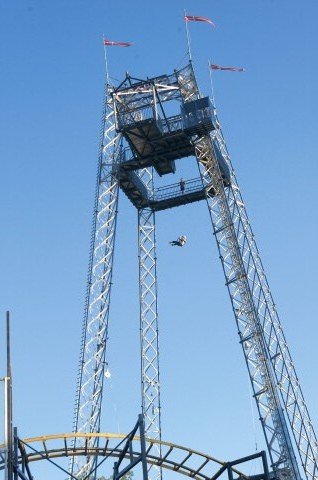
\includegraphics[width=0.5\linewidth]{Sky_Tower.jpg}
\end{center}
\end{minipage}

